\documentclass[sigconf]{acmart}

\usepackage{balance}
\usepackage{graphicx}

\usepackage{url}
\usepackage{amsmath}
\usepackage{mathtools}
\usepackage{tabularx}

\usepackage{caption}
\usepackage{subcaption}

\usepackage{multirow}

\usepackage{graphics}

\begin{document}

    \title{Sample Latex File}
    \author{David P. Little}
    \date{26 August 2018}
    \maketitle
\begin{abstract}
    ply dummy text of the printing and typesetting industry. Lorem Ipsum has been the industry's standard dummy \label{intro} text ever since the 1500s, when an unknown printer took a
    galley of type and scrambled it to make a type specimen book.ply dummy text of the printing and typesetting industry. Lorem Ipsum has been the industry's standard dummy \label{intro} text ever since the 1500s, when an unknown printer took a
    galley of type and scrambled it to make a type specimen book.ply dummy text of the printing and typesetting industry. Lorem Ipsum has been the industry's standard dummy \label{intro} text ever since the 1500s, when an unknown printer took a
    galley of type and scrambled it to make a type specimen book.ply dummy text of the printing and typesetting industry. Lorem Ipsum has been the industry's standard dummy \label{intro} text ever since the 1500s, when an unknown printer took a
    galley of type and scrambled it to make a type specimen book.ply dummy text of the printing and typesetting industry. Lorem Ipsum has been the industry's standard dummy \label{intro} text ever since the 1500s, when an unknown printer took a
    galley of type and scrambled it to make a type specimen book.
\end{abstract}
\section{First Section}

    But I must explain to \textbf{bold text inserted here} you how all  this mistaken idea of denouncing pleasure and praising pain was
    born and I will give you a
    \begin{center}
    complete account of the system, and expound the actual teachings of the great explorer of the truth, the master builder of human happiness. No one rejects, dislikes, or avoids pleasure itself, because it is pleasure, but because those who do not know how to pursue pleasure rationally encounter consequences that are extremely painful. Nor again is there anyone who loves or pursues or desires to
    obtain pain of itself, because it is pain, but because \underline{occasionally circumstances occur} in which toil and pain can procure him some great pleasure.
    To take a trivial example, which of us ever undertakes laborious physical exercise, except to obtain some advantage from it?
    \end{center}
    But who has any right to
    find fault with a man who chooses to enjoy a pleasure that has no annoying consequences, or one who avoids a pain that produces no resultant pleasure?
    \section{What is Lorem Ipsum?}

    \textbf{Lorem Ipsum} is simply dummy text of the printing and typesetting industry. Lorem Ipsum has been the industry's standard dummy \label{intro} text ever since the 1500s, when an unknown printer took a
    galley of type and scrambled it to make a type specimen book. It has survived not only five centuries, but also
    the leap into electronic typesetting, \textit{remaining essentially unchanged}. It was popularised in the 1960s with the release of Letraset sheets containing Lorem Ipsum passages, and more
    recently with desktop publishing software like Aldus PageMaker including versions of Lorem Ipsum.
    \begin{figure}
    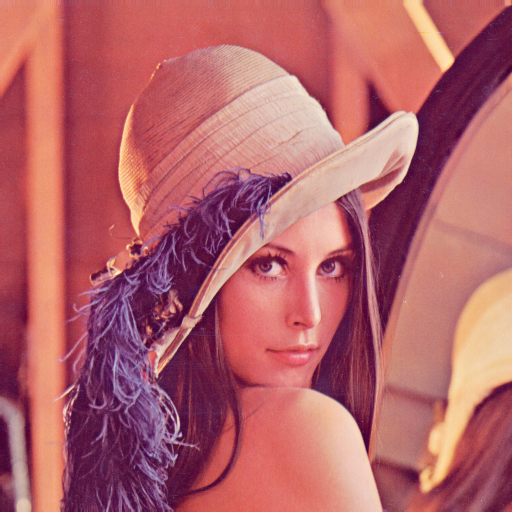
\includegraphics[width=4cm, height=4cm]{lenna.png}

    \label{sec2}
    \caption{Lenna}

    \end{figure}
    \subsection{Sub Section}
this is subsection. Lorem Ipsum has been the industry's standard dummy  text ever since the 1500s, when an unknown printer took a galley of type and scrambled it to make a type specimen book. It has survived not only five centuries, but also
    the leap into electronic typesetting, \textit{remaining essentially unchanged}. \par It was popularised in the 1960s with the release of Letraset sheets containing Lorem Ipsum passages, and more
    recently with desktop publishing software like Aldus PageMaker including versions of Lorem Ips

\begin{itemize}
\item Roger Federer
\item Rafael Nadal
\item Novak Djokovic
\end{itemize}
\subsection{Second Sub Section}
    asfs Hello how are you \\
second line of section   and the text continue ..

    \section{Work Done}
    Following parts of Latex can be successfully converted by this code:
    \begin{enumerate}
        \item title
        \item author
        \item date
        \item maketitle
        \item section
        \item subsection
        \item itemize
        \item enumerate
        \item textbf
        \item textit
        \item includegraphics
        \item   sum
        \item sqrt
        \item frac
        \item inlinemath
        \item displaymath
    \end{enumerate}

    \subsection {Example of Tabular Environment}
    The ranking of men's single ahead of US Open 2018. \\

        \begin{tabular}{|c|c|c|}

            Player & Country & Rank & Test & Test column 2 \\
            Rafael Nadal & Spain & 1 & 2.2345 & 2.678 \\
            Roger Federer & Switzerland & 2 & Country & Rank  \\
            Novaj Djokovic & Serbia & 2 & Country & Rank  \\

            Rafael Nadal & Spain & 1 & & &  \\
            Roger Federer & Switzerland & 2 & & &  \\
            Novaj Djokovic & Serbia & 2 & & & \\

        \end{tabular}


    \subsection{Example of Maths}

    The mass-energy equivalence is described by the famous equation and you can go to figure \ref{sec2}
    $$E=mc^2$$
    $$f(x) =  \sum_{i=0}^{n} (i^2+i+10)  $$
    $$x_2 - 5 x + 6 = 0$$
    $$f(x)= \int_{a}^{b} x* \frac{AB}{xyz}dx$$
    $$f(x)= \int xy dx$$
    $$f(x)= \frac{\sqrt{x}}{21} $$




\end{document}
